%!TEX TS-program = xelatex

% Официальный шаблон презентации НИУ ВШЭ в beamer (LaTeX)
% Версия 2.0
% Язык — русский   
% Автор шаблона - Данил Фёдоровых (fedorovykh@gmail.com)

%%% Для корректной работы шаблона необходима 
%%% установка в систему бесплатного шрифта HSE Sans
%%% https://www.hse.ru/info/brandbook/#font


\documentclass[aspectratio=169]{beamer}

\newbool{russian}
\booltrue{russian}  % Загружает русскоязычный логотип ВШЭ
\usepackage{HSE-theme/beamerthemeHSE} % Подгружаем тему

%%% Работа с русским языком и шрифтами
\usepackage[english,russian]{babel}   % загружает пакет многоязыковой вёрстки
\usepackage[no-math]{fontspec}      % подготавливает загрузку шрифтов Open Type, True Type и др.
	\setsansfont{HSE Sans} 
	\setmonofont{Courier New}
\usepackage{mathspec}
	\setmathsfont(Digits,Latin,Greek)[Numbers={Lining,Proportional}]{HSE Sans}
	\setmathrm[Numbers={Lining,Proportional}]{HSE Sans}
\uselanguage{russian}
\languagepath{russian}
\deftranslation[to=russian]{Theorem}{Теорема}
\deftranslation[to=russian]{Definition}{Определение}
\deftranslation[to=russian]{Definitions}{Определения}
\deftranslation[to=russian]{Corollary}{Следствие}
\deftranslation[to=russian]{Fact}{Факт}
\deftranslation[to=russian]{Example}{Пример}
\deftranslation[to=russian]{Examples}{Примеры}

\usepackage{blindtext} 		% Случайный текст
\graphicspath{{images/}}  	% Папка с картинками
\usepackage{caption}
\captionsetup[figure]{labelsep=period, labelformat=empty}

%%% Информация об авторе и выступлении
\title[Заголовок]{Шутки в сторону: машинное обучение и интерпретируемый искусственный интеллект в задачах генерации юмористических текстов} 
\author[Имя автора]{Король Михаил БПМИ2310, 2 курс \\ \smallskip \scriptsize \url{mkorol@hse.ru} \\{Научный руководитель: д.ф.-м.н. профессор Громов В.А.}}
\institute{Факультет компьютерных наук}
\date{22 апреля 2025 г.}

\begin{document}	% Начало презентации

\frame[plain]{\titlepage}	% Титульный слайд

\begin{frame}
\frametitle{Введение}
\framesubtitle{Актуальность, цель и гипотеза}
	В данный момент ИИ не умеет генерировать юмор. Точнее, из множества сгенерированных шуток, довольно низкий процент окажется действительно смешным. Несмотря на большое количество работ, посвященных теме генерации юмора и юмору в целом, он остается одним из самых сложных явлений для понимания и формализации с точки зрения науки. 
\newline
\newline
	Цель: найти качественные различия между обычными и юмористическими текстами для создания методов их автоматической классификации.\\
	Гипотеза: существуют фундаментальные различия в структуре языка, используемого в юмористических и литературных текстах, которые могут быть выявлены и количественно описаны с помощью методов теории хаоса и топологического анализа.
	
\end{frame}

\begin{frame}
\frametitle{Литературный обзор}
\framesubtitle{Топологический анализ}

В статье \cite{gromov_spot_2024} авторы исследуют структуру естественного языка с целью различения текстов, написанных человеком, и текстов, созданных ботами. Для понимания структуры языков авторы собирают словари эмбеддингов, после этого по взятым текстам строятся биграммы, то есть векторизованные два рядом стоящих слова, и производится векторизация Вишарта, авторы используют несколько метрик для оценки кластеризации, после чего статистически доказывают различие в структуре текстов, написанных людьми, и текстов, написанных ботами. Было бы интересно использовать эту методику для проверки гипотезы о том, что структура юмора и литературных текстов имеет статистически значимые семантические различия.


\end{frame}

\begin{frame}
\frametitle{Литературный обзор}
\framesubtitle{Теория хаоса}

В статье \cite{gromov_semantic_2023} в качестве цели предполагается доказать, что семантические траектории являются хаотическими рядами. Рассматривая слова как векторы, мы хотим изучать тексты как пути динамической системы в фазовом пространстве. Семантическая траектория как раз является таким путем. \\
В статье вводится метод плоскости Энтропия-Сложность, с помощью которого авторы показывают, что семантическая траектория действительно является хаотичным рядом. Рассматривая юмористические тексты, можно применить этот метод для семантических траекторий в юморе, сделать выводы, к каким последовательностям они относятся, а так же понять, есть ли на этой плоскости явное различие между литературными текстами и юмором.

\end{frame}

\begin{frame}
\frametitle{Методология}
\framesubtitle{Плоскость Энтропия-Сложность}

Мартин, Пластино и Россо (MPR) \cite{rosso_distinguishing_2007} предлагают подход, позволяющий отличить хаотический ряд от ряда, генерируемого простой детерминированной системой, и от ряда, генерируемого случайным образом. Чтобы использовать такой метод, нужно как-то представить наши тексты в виде временного ряда. Собран корпус анекдотов и корпус литературы. Произведена базовая обработка корпусов, которая включает в себя очистку данных и лемматизацию. \\
Далее с помощью словаря эмбедингов получаем ряд векторов. 
	
\end{frame}

\begin{frame}
\frametitle{Методология}
\framesubtitle{Плоскость Энтропия-Сложность}
	Рассмотрим наблюдаемую часть временного ряда $ y_0, y_1, \dots, y_t, \dots $ и разобьем его на отрезки длины $k$. В теории их называют z-векторы.
	$$ 
	z_0 = (y_0, y_1, \dots, y_{k-1}) 
	$$
	$$
	z_1 = (y_1, y_2, \dots, y_{k}) 
	$$
	И так далее. Обычно $k$ - небольшая величина. Чтобы ее оценить, можно воспользоваться методом ложных ближайших соседей, добавляя условие на выполнение теоремы Таккенса \cite{rand_detecting_takkens_1981}: размер z-векторов 𝑚 должен удовлетворять условию $m > 2d + 1$, где $d$ — размерность аттрактора. Подробнее см. отчет стр. 6.  \\
	Суть метода заключается в вычислении двух величин, основываясь на полученных вероятностях, характеризующих исходный временной ряд.

\end{frame}

\begin{frame}
\frametitle{Методология}
\framesubtitle{Плоскость Энтропия-Сложность}
	Первая величина -- это привычная нам энтропия, но нормированная на ее максимальное значение ($log \text{ } m$)
	
	$$
	0 \leq H \leq 1 
	$$
	
	Вторая характеристика носит название сложности, а если быть точным, MPR-сложности (которая названа по первым буквам фамилий ее авторов).

	$$ 
	C_{\text{MPR}} = Q_0 \cdot H \cdot \|P - P_e\| 
	$$
	
	где $P_e - $ равномерное распределение, то есть: $P_e = \{p_j = 1/N\}$, $H$ -- энтропия, \\ $ Q_0$ -- нормализирующая константа, которая гарантирует, что $0 \leq C_{\text{MPR}} \leq 1$, $\|P - P_e\|$ показывает, насколько уклоняется актуальное распределение от распределения равномерного.
\end{frame}

\begin{frame}
\frametitle{Методология}
\framesubtitle{Плоскость Энтропия-Сложность}
	Благодаря этим двум характеристикам получается следующая картина: \\ 
	 \begin{figure}[htbp]
            \centering
            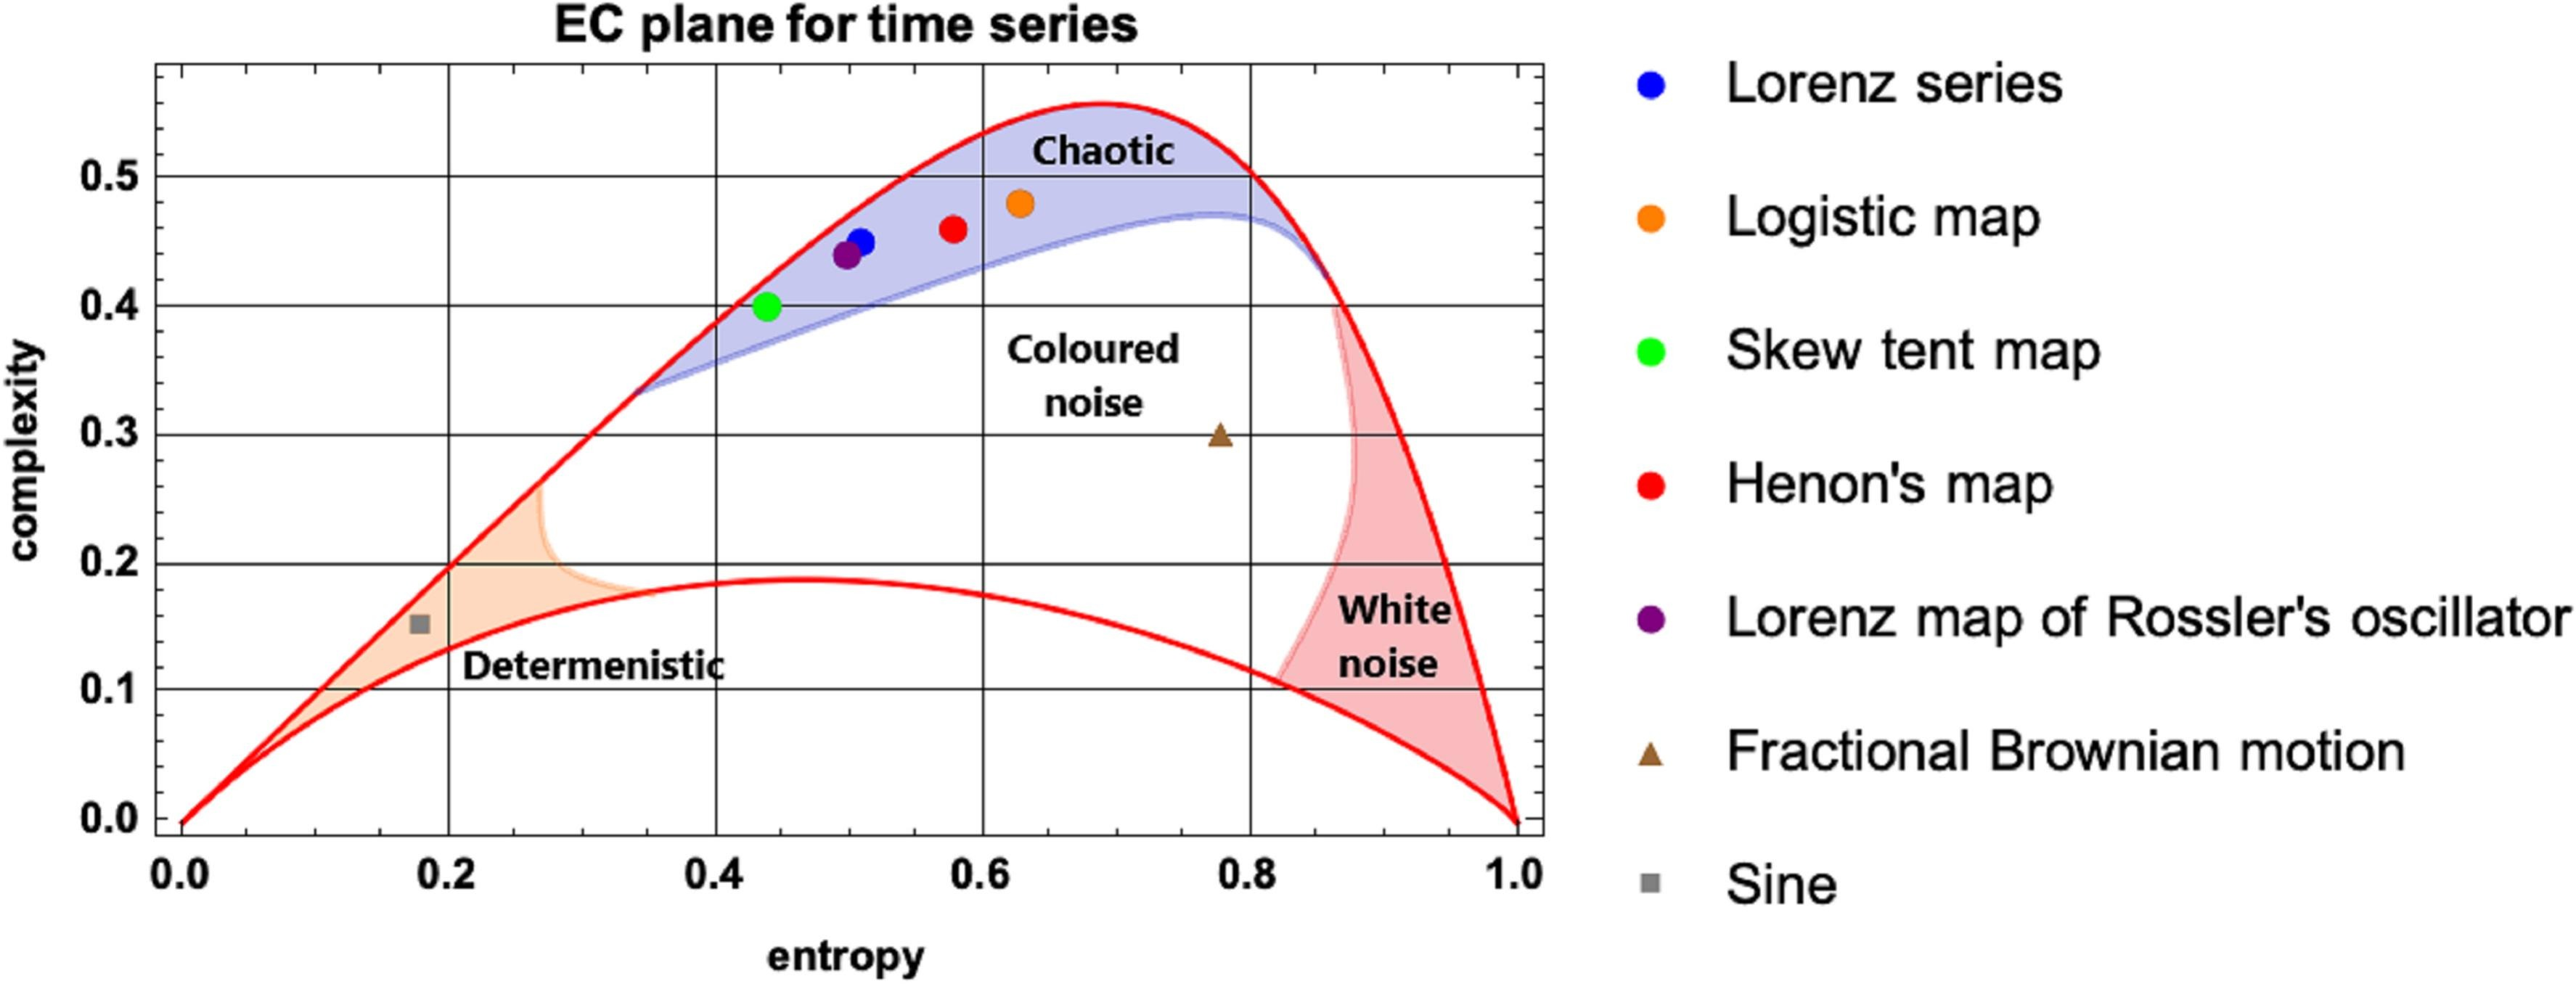
\includegraphics[scale=0.6]{image2}
            \caption{Теоретические границы плоскости Энтропия-Сложность}
            \label{fig:image2}
        \end{figure}

\end{frame}

\begin{frame}
\frametitle{Методология}
\framesubtitle{Кластеризация Вишарта}

Для анализа семантических путей будем использовать кластеризацию Вишарта\footnotemark[1] \cite{wishart_numerical_1969}. Этот метод был выбран на основе экспериментов, проведенных в исследовании \cite{gromov_spot_2024}, где он показал высокую эффективность на похожей задаче. Для оценки качества кластеризации будем использовать индекс Калински-Харабаша\footnotemark[2] (CH), который выглядит как:

$$
CH_{\text{adj}} = \left( CH \times \text{ratio\_not\_noise} \right)^T
$$

Где $T$ является гиперпараметром, а $\text{ratio\_not\_noise}$ — количество точек, помеченных как шум, поделенный на общее количество точек.

\footnotetext[1]{\url{github.com/quynhu-d/stb-semantic-analysis-tools/blob/main/lib/clustering/WishartParallelKD.py}}
\footnotetext[2]{\url{scikit-learn.org/stable/modules/generated/sklearn.metrics.calinski_harabasz_score.html}}

\end{frame}

\begin{frame}
\frametitle{Экспериментальное исследование}
\begin{itemize}
	\item Был собран датасет шуток, содержащий около 90 тыс. анекдотов на разную тематику с различных источников. 
	\item Эмбеддинги были получены через методы SVD и CBOW, словари эмбеддингов были взяты в лаборатории.
\end{itemize}
\end{frame}

\begin{frame}
\frametitle{Экспериментальное исследование}
\framesubtitle{Плоскость Энтропия-Сложность}

	\begin{columns}
	 \column{0.5\textwidth}
	 С помощью метода ложных соседей были оценены размеры z-векторов. Результат вычислений совпал со значениями, которые использовались в статье \cite{gromov_semantic_2023}, авторы в итоге рассматривали значения $n = 2, m = 7 - 8$, а так же $n = 3, m = 4 - 5$. Остальные значения уходили либо в шум, либо в детерменированные процессы. \\ Сначала был воспроизведен результат из самого исследования $\rightarrow$
	\column{0.5\textwidth}
	\begin{figure}[htbp]
            \centering
            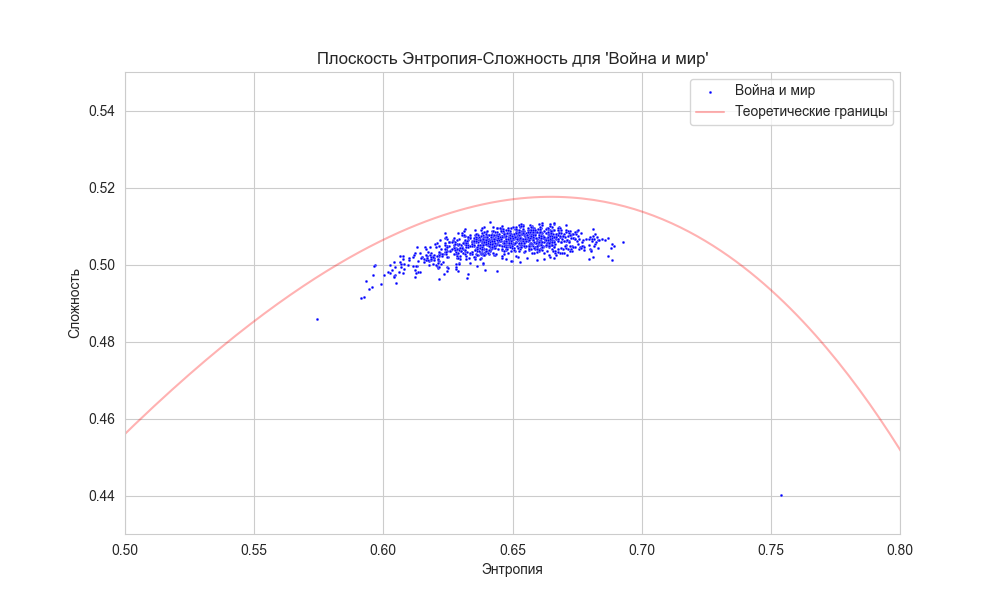
\includegraphics[scale=0.26]{image3}
            \caption{Расположение "Война и мир" на плоскости Энтропия-Сложность}
            \label{fig:image3}
        \end{figure}
	\end{columns}
	
\end{frame}

\begin{frame}
\frametitle{Экспериментальное исследование}
\framesubtitle{Плоскость Энтропия-Сложность}
	
	\begin{figure}[htbp]
            \centering
            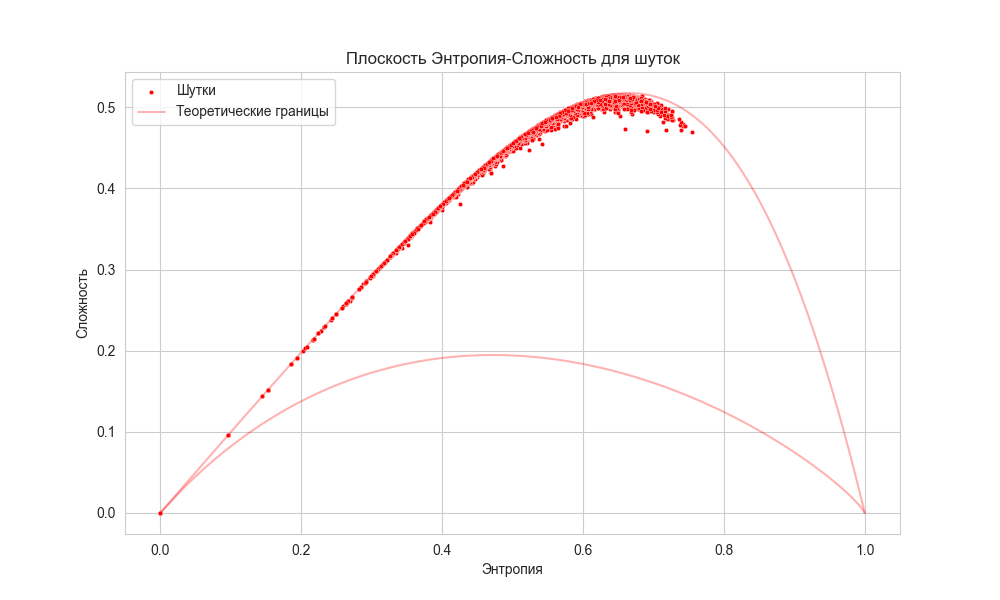
\includegraphics[scale=0.4]{image7}
            \caption{Расположение шуток на плоскости Энтропия-Сложность}
            \label{fig:image1}
        \end{figure}

\end{frame}

\begin{frame}
\frametitle{Экспериментальное исследование}
\framesubtitle{Плоскость Энтропия-Сложность}
	
	\begin{figure}[htbp]
            \centering
            
\includegraphics[scale=0.4]{image1}
            \caption{Расположение данных на плоскости Энтропия-Сложность}
            \label{fig:image1}
        \end{figure}

\end{frame}

\begin{frame}
\frametitle{Экспериментальное исследование}
\framesubtitle{Плоскость Энтропия-Сложность}
	
	\begin{figure}[htbp]
            \centering
            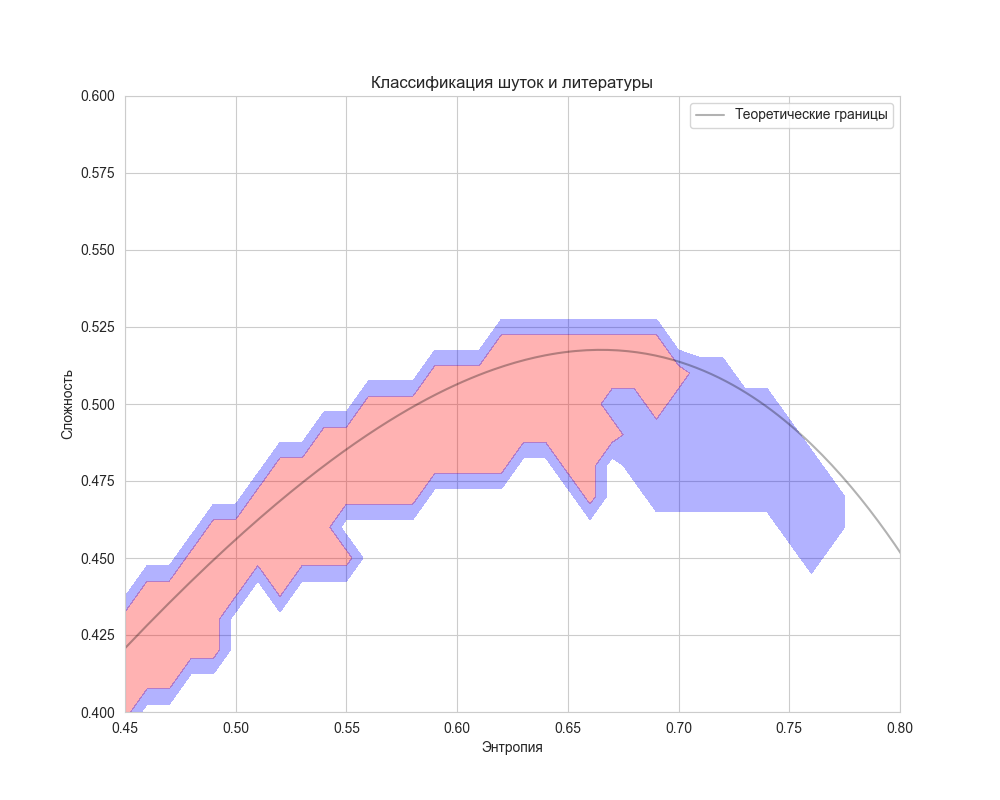
\includegraphics[scale=0.3]{image6}
            \caption{Классификатор}
            \label{fig:image6}
        \end{figure}

\end{frame}

\begin{frame}
\frametitle{Экспериментальное исследование}
\framesubtitle{Плоскость Энтропия-Сложность}
	
	\begin{figure}[htbp]
            \centering
            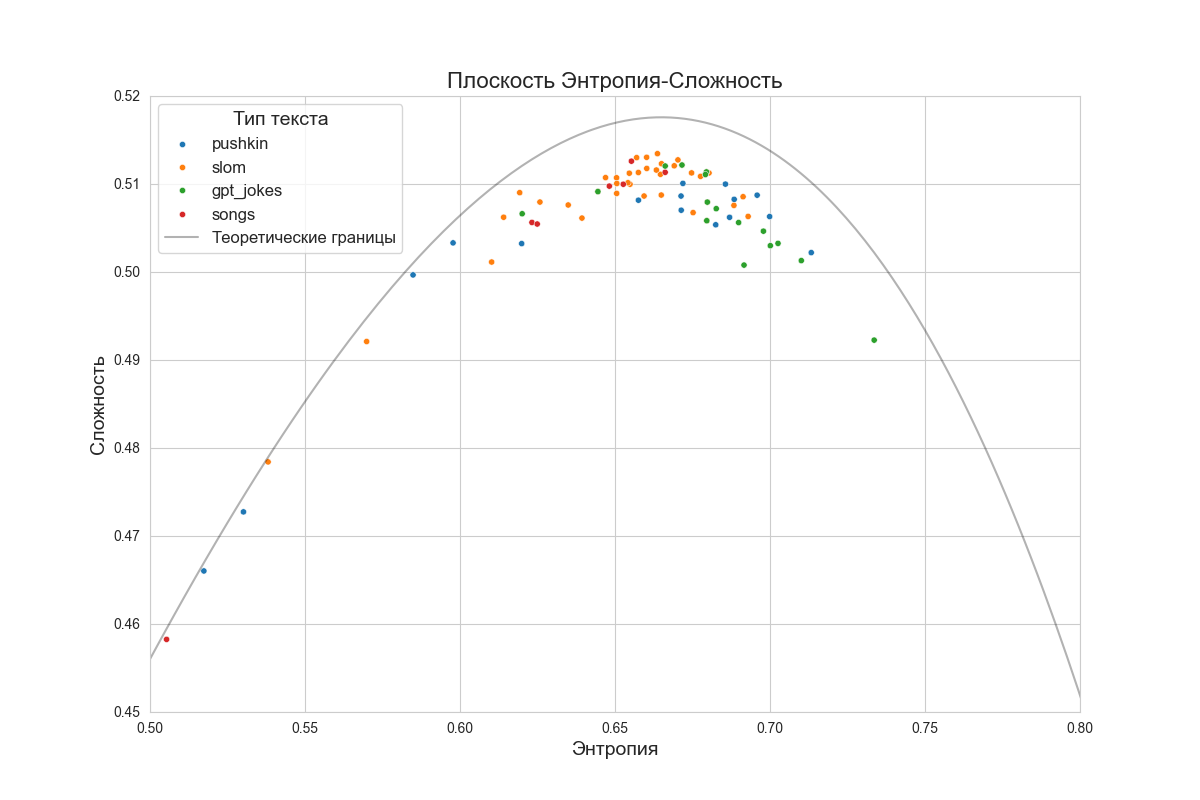
\includegraphics[scale=0.3]{image8}
            \caption{Различные категории текстов}
            \label{fig:image6}
        \end{figure}

\end{frame}

\begin{frame}
\frametitle{Заключение}
\framesubtitle{Дальнейшее развитие}

Данная работа имеет большой потенциал для дальнейших исследований. Семантическое пространство не было рассмотрено должным образом из-за проблем с кластеризацией. Были подготовлены данные для кластеризации, изучена библиотека t-SNE. Можно расширить методологию за счет большего количества уникальных языковых данных. 
\newline
\newline
Вывод: различие действительно есть, но его недостаточно.
\end{frame}

\begin{frame}
\frametitle{Библиография}
	\bibliographystyle{apalike} 
	\bibliography{course_work_humor} 
\end{frame}

\begin{frame}
\frametitle{Приложения}
	\url{github.com/DogeSavior3/shutki-v-storonu}
\end{frame}


\end{document}